\begin{figure}[!t]
  \center {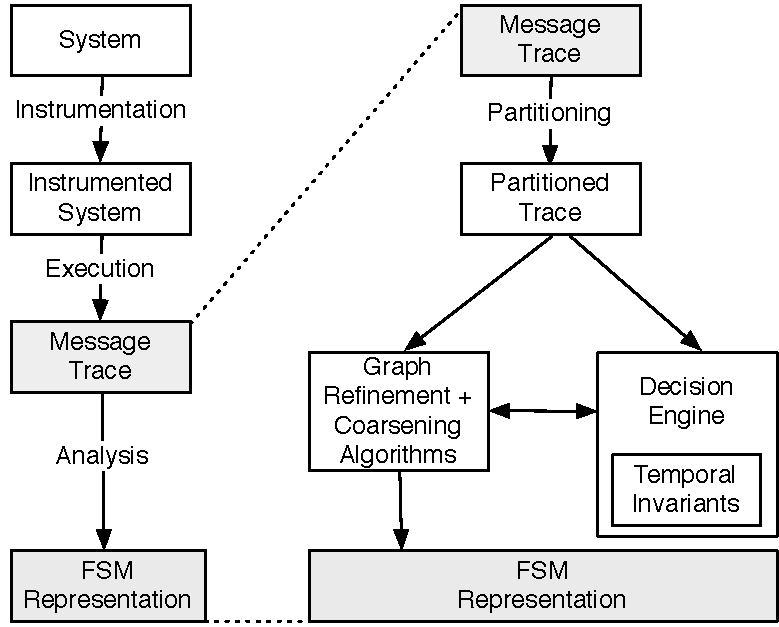
\includegraphics[scale=.6]{img/joined_design.pdf}}
  \caption{An overview of the system pipeline (left) and the details
    of the analysis pipelines implementing (right).}
  \label{fig:design}
\end{figure}

%%%%%%%%%%%%%%%%%%%%%%%%%%%%%%%%%%%%%%%%%%%%%%%%%%%%%%%%%%%%%%%%%%%%%
\section{System Design}
\label{sec:design}
%%%%%%%%%%%%%%%%%%%%%%%%%%%%%%%%%%%%%%%%%%%%%%%%%%%%%%%%%%%%%%%%%%%%%

Synoptic is comprised of several components. Figure~\ref{fig:design}
illustrates these components, and in the rest of this section we
briefly overview each of them.

Synoptic starts by inferring a set of temporal properties between
messages in the trace. Synoptic then runs either the coarsening or the
refinement algorithm to derive a FSM representation of the trace,
which is presented to the user. 

%%%%%%%%%%%%%%%%%%%%%%%%%%%%%%%%%%%%%%%%%%%%%%%%%%%%%%%%%%%%%%%%%%%%%
\subsection{Message Capture}
%%%%%%%%%%%%%%%%%%%%%%%%%%%%%%%%%%%%%%%%%%%%%%%%%%%%%%%%%%%%%%%%%%%%%

To be used with Synoptic, the input system must be manually modified
to capture all network-level messages. We use the term \emph{message}
in a general sense to refer to a formatted message sent between two
nodes in a distributed system.

There are several ways to capture messages
(section~\ref{sec:discussion} discusses some alternatives). The core
of Synoptic is independent of how the messages are captured, and in
our evaluation (section~\ref{sec:evaluation}) we study systems whose
messages are captured in a variety of ways. We assume that the the end
result of message capture process is a trace that has the following
structure:

\begin{align*}
\left<\textup{src}, \textup{dst}, \textup{timestamp}, \left[datafields\right]\right>
\end{align*}

For example a three way handshake trace could look like the following
sequence of six messages:

\begin{align*}
\left<\textup{1}, \textup{2}, \textup{0}, \left[REQ\right]\right>\\
\left<\textup{2}, \textup{1}, \textup{1}, \left[RESP\right]\right>\\
\left<\textup{1}, \textup{2}, \textup{2},  \left[ACK\right]\right>\\
\left<\textup{3}, \textup{2}, \textup{3}, \left[REQ\right]\right>\\
\left<\textup{2}, \textup{3}, \textup{4}, \left[RESP\right]\right>\\
\left<\textup{3}, \textup{2}, \textup{5},  \left[ACK\right]\right>
\end{align*}

Each message must include extra meta information such as the source
and destination node addresses above. Because we assume that messages
are never lost (see section~\ref{sec:assumptions}), we only capture
outgoing messages. The node traces are then manually collected and
manually merged into a single trace. To make this feasible, we assume
that the nodes use NTP or a similar protocol to synchronize their
local time.

%%%%%%%%%%%%%%%%%%%%%%%%%%%%%%%%%%%%%%%%%%%%%%%%%%%%%%
\subsection{Analysis}
%%%%%%%%%%%%%%%%%%%%%%%%%%%%%%%%%%%%%%%%%%%%%%%%%%%%%%

The analysis component is the core of Synoptic. To perform analysis,
the user must first manually create semantically meaningful partitions
of the message trace. Second, the user must specify one of two
algorithms Synoptic should use -- GK-Tail, or Bikon. Depending on the
algorithm, Synoptic then converts the input message trace into one of
two FSM representations. The first representations is more direct as
it makes no assumption about the structure of the underlying
process. The second representation is more intuitive to systems
designers. Either of the representations can be converted to the
other.

Next, Synoptic explores the set of possible FSM representations until
it finds one that satisfies certain constraints. Depending on the
algorithm, this exploration takes the form of either refinement or
coarsening of the FSM. Coarsening starts with a concrete
representation of the partitioned trace and merges states to derive
smaller representations. Refinement starts with a single state
representing all messages of the same type in a partition trace, and
enlarges the representations by splitting these states. Finally, the
end result of this exploration is displayed to the user as an FSM
image.

%%%%%%%%%%%%%%%%%%%%%%%%%%%%%%%%%%%%%%%%%%%%%%%%%%%%%%
\subsubsection{Trace Partitioning}
%%%%%%%%%%%%%%%%%%%%%%%%%%%%%%%%%%%%%%%%%%%%%%%%%%%%%%

The final manual step performed by the user is trace
partitioning. This groups messages into instances of the process that
generated the messages. Partitioning is necessary to limit the scope
relations between messages in the trace. Its also necessary to tease
apart concurrent protocols. As a general rule, messages that are
generated independently should belong to different partitions.

The choice of partition function is crucial to derive a proper
representation for the traces. For example, the two-phase commit
protocol traces used in the evaluation are partitioned by run of the
system -- each complete execution of the protocol is a unique
trace. Another partitioning scheme might partition the global trace by
node, so that the resulting representation captures a single node's
perspective of the system.

For this step we use a set of partitioning predicates $p_1,...,p_n$,
such that for every message exactly one predicate is true. If
predicate $p_i$ is true for a message $m$, we say message $m$ has type
$i$. The partitioning predicates are assumed to be supplied by the
user.

%%%%%%%%%%%%%%%%%%%%%%%%%%%%%%%%%%%%%%%%%%%%%%%%%%%%%%
\subsubsection{Interpreting Traces as Graphs}
%%%%%%%%%%%%%%%%%%%%%%%%%%%%%%%%%%%%%%%%%%%%%%%%%%%%%%

Synoptic employs two different models to interpret the partitioned
messages as directed graphs. The first assumes as little as possible
about the process that generated the messages, and relates messages
according to their properties. The second model considers the messages
as being generated by a system that may or may not transition between
different states each time a message is sent or received. As we will
show, the representations of these models are equivalent. Next we
formally define these representations, and show them to be equivalent.

\paragraph{Messages are temporally related.} The first model captures
how message relate according to their properties. The relation we use
is time (i.e. message X follows message Y). However, there are other
relations such as is-response (i.e. message X is a response to message
Y). Given a trace of messages $M$, Synoptic constructs a graph $G =
(V, E)$, in which vertices represent sets of messages:

\begin{align*}
  V~=~&\mathcal{P}(M)
\end{align*}

We choose sets of messages to allow flexibility that we will need
later on. For now, we only relate singleton sets of vertices according
to the the time relation $t$:

\begin{align*}
E~=~&\{(\{m_1\},\{m_2\},t)~|~m_1,m_2\in{M}\wedge{}\\
	&m_1.tstamp < m_2.tstamp\}
\end{align*}

% For the trace above, this model produces the representation in
% Figure~\ref{fig:gk_tail_ex_representation}.

\paragraph{Messages transform System State} The second model
associates each message with a system state that produced the
message. Given a message trace $M$, Synoptic constructs a graph $G =
(V, E)$ in which every vertex represents some notion of \textit{system
  state}. Since we assume the input trace to be linear, we need
$|M|+1$ states. We can use the natural numbers $[1,|M|+1]$ as states,
but for flexibility we use sets of natural numbers:

\begin{align*}
V~=~&\{\{i\}~|~i\in[1,|M|+1]\}\\
\end{align*}

We now want to relate states according to the messages that cause the
transition. The fundamental assumption we make here is that if message
$m_1$ occurred immediately before message $m_2$ in the trace, then
$m_1$ caused the system to enter the state associated with $m_2$. We
capture this by interpreting $m_1$ as a transition from the system
state associated with $m_1$ to the system state associated with
$m_2$. Since we required the \texttt{tstamp} fields to be distinct in
every trace, ordering the set $\{m.tstamp~|~m\in{M}\}$ yields a
sequence $s_1,\dots,s_{|M|}$ of length $|M|$. We are now ready to
construct the set of edges E:

\begin{align*}
E~=~&\{(\{i\},\{i+1\},m)~|~m\in{M}\wedge{}s_i=m.tstamp\}
\end{align*}

In other words, we order the messages chronologically, and create
states between them. For consistency we use this system-state
representation throughout the paper.

%  For the trace above, this model produces the
% representation in
% Figure~\ref{fig:bikon_ex_representation}.\\

\paragraph{Relating the representations}

\begin{figure}[t]
\centering
\subfloat[Relational
representation]{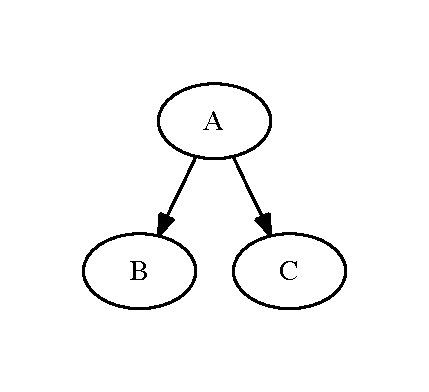
\includegraphics[width=1.5in]{img/bisim_to_gktail1.pdf}}
\hspace{.4in}
\subfloat[System state representation]{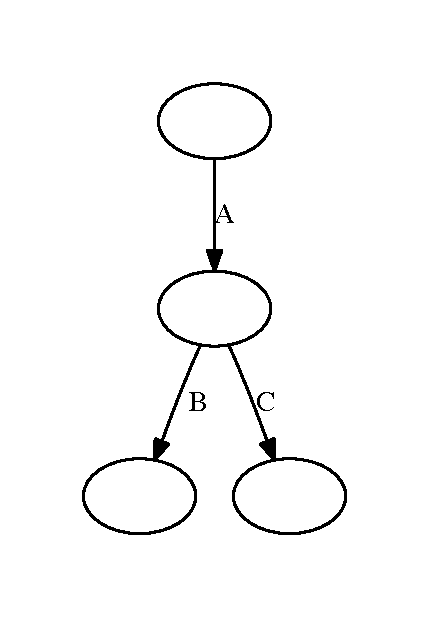
\includegraphics[width=.9in]{img/bisim_to_gktail2.pdf}}
\caption{An example to illustrate automated conversion of a relational
  representation in \textbf{(a)} to the system state representation in \textbf{(b)}.}
\label{fig:bisim_to_gktail}
\end{figure}

Let $G=(V,E)$ be a graph that interprets messages as states. Then we
can construct a graph $G'=(V',E')$ that interprets messages as
transitions and allows the same traces. Let $V=\{s_1,...,s_n\}$ and
$r$ be a relation according to which we will perform the
translation. Then $G'$ can be constructed as follows:

\begin{align*}
V'~=~	&\{0,...,n\}\\
E'~=~	&\{(i,j,s_j)~|~(s_i,s_j, r)\in{E}\}\cup\\
 	&\{(0,i,s_i)~|~\neg\exists{j}:~(s_j,s_i)\in{E}\}
\end{align*}

As an example of this conversion, consider
Figure~\ref{fig:bisim_to_gktail}. In graph \textbf{(a)}, G is
represented in the relational form, while in \textbf{(b)} the same
graph is represented in terms of system states.

%We found it useful to view representations in the
%messages-as-transitions form as describing a dynamic system state in
%terms of the messages that can be sent or received.

We are also fairly confident that the reverse translation is also
possible, at least for the chosen translation relation. It is also
apparent that interpreting messages as states yields a more general
representation, as it allows for a variety of different relations
between messages.


%%%%%%%%%%%%%%%%%%%%%%%%%%%%%%%%%%%%%%%%%%%%%%%%%%%%%%%%%%%%%%%%%%%%%
\subsubsection{FSM Representations Exploration}
%%%%%%%%%%%%%%%%%%%%%%%%%%%%%%%%%%%%%%%%%%%%%%%%%%%%%%%%%%%%%%%%%%%%%

\begin{figure}[t]
  \center
  {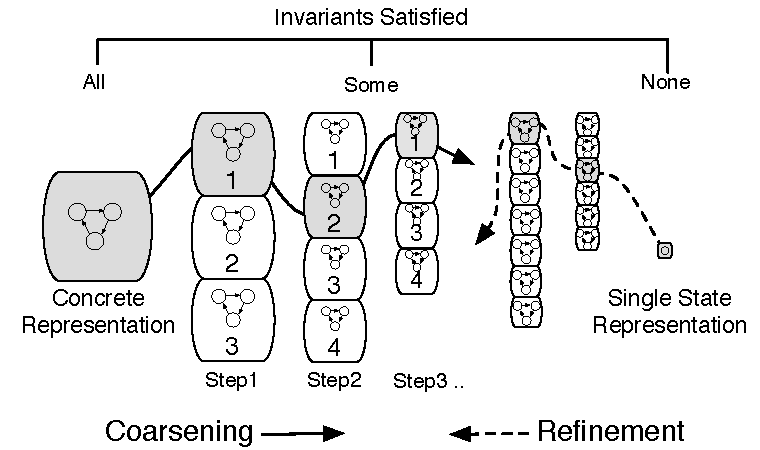
\includegraphics[width=\columnwidth]{img/refine_coarsen.pdf}}
  \caption{Coarsening and Refinement are dual operations on the graph
    representation. Squashed rectangles denote intermediate FSM
    representation, and the size of the squashed rectangle denotes
    representation size (e.g. number of states and transitions in the
    FSM graph). The most compact representation is a single state
    representation, while the least compact representation is the
    concrete representation. Refinement starts with a single state
    representation and can proceed (to the left) until the concrete
    representation is achieved. Coarsening starts with the concrete
    representation and can proceed (to the right) until a single state
    representation is achieved. Three steps of coarsening are labeled;
    the intermediate representations at each step are shaded squashed
    rectangles. At the top, the representations are related to trace
    invariant satisfaction. All invariants are satisfied in the
    concrete representation, and fewer are satisfied until a single
    state representation is reached, at which point no invariants are
    satisfied.}
 \label{fig:refine_coarsen}
\end{figure}

To explore the space of potential FSM representations Synoptic uses
two dual operations: refinement and coarsening. These are illustrated
in Figure~\ref{fig:refine_coarsen}. A variety of decisions that the
graph refinement and coarsening algorithms have to make are
encapsulated in the decision engine (explained in
section~\ref{sec:decision_engine}). Here we overview the intuition behind
refinement and coarsening.

%%%%%%%%%%%%%%%%%%%%%%%%%%%%%%%%%%%%%%%%%%%%%%%%%%%%%%%%%%%%%%%%%%%%%
\paragraph{Graph Refinement}
%%%%%%%%%%%%%%%%%%%%%%%%%%%%%%%%%%%%%%%%%%%%%%%%%%%%%%%%%%%%%%%%%%%%%

Graph refinement begins by grouping all messages of a particular type
into a single state. The algorithm then starts to find
counter-examples to this grouping, and refines the states
accordingly. State refinement is based on a property that splitting
the messages associated with a state into two sets preserves the
temporal properties of the messages observed in the original trace.

% For example, the behavioral predicates such as \emph{appearing
%   before} could be used, as well as structural predicates such as a
% including a certain data fields or having a field with a value in a
% certain value ranges. This is a possible area to apply
% Daikon~\cite{Daikon} to refinement.

State refinement allows decisions to be made depending on the
properties of the entire partition. For example, if only a small
number of states can be split out, the algorithm can decide not to
split so as to maintain a more compact representation. In general,
statistical measures can be used to drive the refinement (see
discussion in section~\ref{sec:discussion}).

If certain refinements should be guaranteed, the initial graph can
start with a more fine grained initial assignment of messages to
states. At the moment we make the initial assignment based on the
user-supplied message type predicates.

%%%%%%%%%%%%%%%%%%%%%%%%%%%%%%%%%%%%%%%%%%%%%%%%%%%%%%%%%%%%%%%%%%%%%
\paragraph{Graph Coarsening}
%%%%%%%%%%%%%%%%%%%%%%%%%%%%%%%%%%%%%%%%%%%%%%%%%%%%%%%%%%%%%%%%%%%%%

Graph coarsening is the dual operation of graph refinement. The
initial assumption is that all messages are different. When
similarities are detected between some set of states, the states are
merged into a single state while preserving the transitions of the
initial states. A variety of state similarity notions may be used --
behavioral, structural, or both. At the moment we only consider
behavioral properties to decide whether to merge two states or not.

Graph coarsening takes the message type predicates into account and
never merges states with different types. In this way, we achieve the
same restriction as graph refinement.
